\label{ModbusErklärung} \setauthor{Pouget Marcel}
Um die Art der Kommunikation zwischen den Wallboxen, den PV-Anlagen, den Janitza-Klemmen und dem Raspberry PI zu verstehen, muss man sich erstmals mit der Übertragung an sich beschäftigen.
\subsection{7 Schichten OSI-Modell} \label{OsiModell}


Mit dem Open System Interconnection Reference Model (kurz OSI-Referenzmodell) lässt sich am besten beschreiben, wie und auf welchen Ebenen die Daten übertragen werden. Kurz zusammengefasst ist es ein Modell, das die Kommunikation in einem Netzwerk in sieben Schichten unterteilt. Die Entwicklung, welche seit 1983 als Standard veröffentlicht wird, begann bereits 1977. Der Fokus der Entwicklung war es, ein Modell zu erschaffen, mit welchem sich die Kommunikation zwischen Systemen, auch innerhalb eines Netzwerkes, beschreiben lässt. Es gibt dabei sieben Schichten, auf welchen sich unterschiedliche Übertragungsarten abspielen.


Die sieben Schichten des OSI-Modells sind:


\begin{compactenum}
\item Die Bitübertragungsschicht ist die unterste Schicht. Die physische Schicht umfasst die Hardware, die zur Übertragung von Daten über das Netzwerk verwendet wird, wie zum Beispiel verschiedene Kabel (wie Netzwerkkabel, Serielle Verbindungen), Hubs, Switches und Router. Außerhalb eines Netzwerkes könnte die physische Schicht auch der Rauch sein, mit dem Rauchzeichen übermittelt werden, oder die Luft, wenn es um Morsezeichen geht. Im Grunde alles, durch was sich verschlüsselte Nachrichten übermitteln lassen.
\item Ein wichtiger Bestandteil eines Netzwerkes ist die Datenübertragungsschicht. Diese ist verantwortlich für die Übertragung von Datenpaketen von einem Gerät zu einem anderen. Hierbei spielt die MAC-Adresse eine wichtige Rolle, da sie dazu verwendet wird, um einzelne Geräte in einem Netzwerk zu identifizieren. Im Gegensatz zur IP-Adresse besteht die MAC-Adresse aus 48 Bit. Die MAC-Adresse wird in hexadezimaler Form dargestellt, ein Beispiel dafür wäre 00-1D-60-4A-8C-CB. Dabei werden stets zwei Bytes zusammengefasst und durch einen Bindestrich oder durch einen Doppelpunkt getrennt. Die ersten drei Bytes der MAC-Adresse sind die Kennung des Herstellers, welche auch als \glqq OUI\grqq{} bekannt ist. Die restlichen drei Bytes werden von dem jeweiligen Hersteller vergeben und dienen dazu, einzelne Geräte voneinander zu unterscheiden. Das ermöglicht eine eindeutige Identifizierung im Netzwerk und verhindert, dass doppelte MAC-Adressen im Netzwerk vorkommen. Jeder Hersteller muss sich hierfür ein entsprechendes Schema überlegen, um die letzten drei Bytes einer MAC-Adresse eindeutig zu vergeben. \cite{wieisteineMacaufgebaut}
\item Die Netzwerkschicht ist für die Vermittlung von Datenpaketen zwischen Netzwerken verantwortlich und verwendet IP-Adressen, um Geräte im Internet zu identifizieren. \cite{ipAddress} Die klassischen IP4 Adressen bestehen, wie der Name vermuten lässt, aus 4 Bytes und einer Subnetmask. Diese ist dafür da, die Adresse in zwei Teile zu unterteilen. Der vordere Teil repräsentiert dabei immer den Netzwerkteil und der hintere die Computer ID. Für private Netzwerke gibt es reservierte Bereiche. 10.0.0.0/8, was vor allem in großen Firmen benötigt wird, da es 16.777.216 mögliche Adressen gibt. Im Heimnetz kommen vor allem 172.16.0.0/12 und 192.168.0.0/16 vor. Bei diesen IP-Bereichen können in einem Netzwerk viel weniger Geräte genutzt werden. Bei der 172.16.0.0/12 sind es immerhin noch 1.048.576 mögliche Geräte und bei der letzten Möglichkeit nur noch 65.536. Deswegen sind diese in privaten Haushalten am häufigsten zu finden. Ein klassisches Beispiel wäre 192.168.0.100/16.
\item Die Transportschicht ist für die Übertragung von Daten zwischen Endgeräten verantwortlich und sorgt dafür, dass die Übertragung fehlerfrei erfolgt. Auf dieser Schicht kommen vor allem die Protokolle TCP und UDP zum Einsatz. TCP ist dafür da, um mit Hilfe einer Prüfsumme zu gewährleisten, dass alle Daten richtig bei dem Empfänger ankommen. UDP hingegen ist ein auf Geschwindigkeit angelegtes Protokoll, bei dem es auch vorkommen darf, wenn ein paar Bits verloren gehen.
\item Die Sitzungsschicht ist für die Verbindungsaufnahme und-beendigung zwischen Endgeräten verantwortlich und sorgt dafür, dass die Übertragung ordnungsgemäß abläuft.
\item Die Darstellungsschicht ist für die Umwandlung von Daten zuständig. Die Daten werden in ein für die Übertragung geeignetes Format umgewandelt und sorgt dafür, dass die Daten in der richtigen Form, also richtig formatiert, an ihr Ziel gelangen. Auch Kompression und Verschlüsslungen gehören zu dieser Schicht.
\item Die Anwendungsschicht ist die oberste Schicht und ist dafür verantwortlich, mit den Anwendungen kommunizieren zu können. Diese werden auf den Endgeräten ausgeführt. Über diese Schicht wird die Verbindung zu den unteren Schichten hergestellt. Hier werden vor allem Applikationen verwendet, mit denen Daten ausgetauscht werden können. Typische Beispiele sind Webbrowser, E-Mail-Programme oder Nachrichtendienste.
\end{compactenum}\cite{ISO/OSI-Referenzmodell}



Das OSI-Referenzmodell hilft, die Kommunikation in einem Netzwerk zu beschreiben und zu verstehen, indem es die verschiedenen Aspekte der Netzwerkkommunikation in logische Schichten unterteilt. Dies ermöglicht es, Netzwerkprotokolle zu standardisieren und die Kompatibilität von Geräten und Software in verschiedenen Netzwerken zu gewährleisten.


\begin{figure}[h t] \cite{7schichtenModell}
\centering
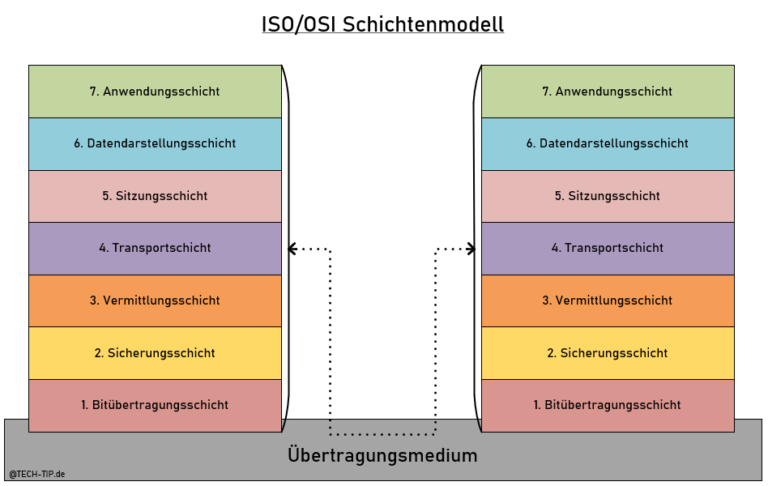
\includegraphics[scale=0.5]{pics/ISO-OSI-Modell-768x486.png}
\caption{Das 7 Schichten OSI/ISO Modell}
\label{fig:impl:Wallbox7schichtenmodell}
\end{figure}



\subsection{Modbus}\label{modbusprotokoll} \setauthor{Pouget Marcel}


Modbus ist ein Protokoll, welches 1979 entwickelt wurde und vor allem in der Industrie große Bedeutung hat. Es ermöglicht eine Kommunikation zwischen automatisierten Maschinen und wurde damals als Protokoll auf der Anwendungsebene implementiert, das Daten über die serielle Schicht übertragen soll. Das Protokoll gehört mittlerweile zu den Industriestandards und wird vor allem in der Automatisierungstechnik gerne benützt. Mittlerweile hat sich Modbus weiterentwickelt, sodass es mehrere Implementierungen gibt. Der Datenaustausch ist mittlerweile über TCP/IP, seriell oder über das 'User-datagram-protocol', kurz UDP, möglich.
\cite{ModbusgrundlagenKubunu} \cite{modbuskubunu}


\subsection{Das Modbus-Protokoll}
Modbus ist ein sogenanntes Request-Response-Protokoll, welches eine 'Master-Slave'-Beziehung nutzt. In so einer 'Master-Slave'-Beziehung funktioniert die Kommunikation immer paarweise – ein Gerät schickt eine Anfrage an einen 'Slave', und wartet auf eine Antwort. Der Master ist dabei für jede Interaktion verantwortlich. Der Master ist normalerweise ein einfaches HMI (human machine interface) oder ein 'Supervisory Control and Data Acquisition (SCADA) System'. Der Slave ist meistens ein Sensor, eine Messklemme, ein programmable logic controller (PLC) oder ein Interface. Der Inhalt der Anfragen und Antworten sowie die Netzwerkschichten, über die diese Nachrichten gesendet werden, werden von den verschiedenen Schichten des Protokolls definiert.
\cite{modbusoverserial}
\subsection{Die verschiedenen Layer des Modbus-Protokolls }
In der ersten Implementierung war Modbus ein einzelnes Protokoll, welches auf serielle Protokolle aufbaut, es konnte also nicht in mehrere Schichten aufgeteilt werden. (Modbus RTU)
Über einen längeren Zeitraum wurden neue Implementierungen vorgestellt, um entweder das serielle Paketformat zu ändern oder die Verwendung von TCP/IP- und UDP-Netzwerken (User Datagram Protocol) zu ermöglichen. TCP, Remote Terminal Unit (RTU) und ASCII sind die drei am häufigsten verwendeten ADU-Formate. RTU- und ASCII-ADUs werden traditionell über eine serielle Verbindung verwendet, während TCP über zeitgenössische TCP/IP- oder UDP-IP-Netzwerke verwendet wird.



\subsection{Aufbau des Modbus-Protokolls}
Am Anfang ist es wichtig zu erwähnen, dass jeder einzelne Teilnehmer (Slave) eine sogenannte Slave-Id besitzt. Diese muss in einem 'Netzwerk' eindeutig identifizierbar sein und kann je nach Hersteller fest vergeben, automatisch konfiguriert oder frei wählbar sein. Die Adresse 0 ist für den Master reserviert. Die einzelnen Teilnehmer können die Adressen von 1 bis 247 annehmen, da die Adressen von 248 bis 255 reserviert sind. Die Daten von den Slaves sind in sogenannten Registern gespeichert. Diese sind immer 16 Bit groß.


Das Protokoll Modbus überträgt die Daten in binärer Form. Das führt dazu, dass die Daten nicht direkt ausgewertet werden können, sondern dass eine Möglichkeit des Parsens gebraucht wird, um auf die ursprünglichen Werte zu kommen. Vorteil ist jedoch, dass dadurch ein großer Datendurchsatz ermöglicht wird.




Soll nun ein Paket über Modbus geschickt werden, müssen zuerst ein paar variable Einstellungen getroffen werden. So kann die Baudrate (Bitrate) oft frei gewählt werden (solange sie nicht von dem Hersteller festgelegt wurde, wie es bei den Wallboxen der Fall war). Außerdem gibt es sogenannte 'Stopbits', welche bei jedem Hersteller anders konfiguriert sind. Die Defaultwerte sind dafür 1 oder 2 Bits.





Vor und nach jedem gesendeten Paket gibt es eine Sendepause (Wartezeit) von mindestens 3.5 Zeichen. Da ein Zeichen eine Länge von 11 Bit besitzt, hängt die Wartezeit von der Bitrate ab. Dabei ist zu beachten, dass vor allem bei einer niedrigen Übertragungsrate es sehr wichtig ist, diese Zeit genau einzuhalten, da es sonst zu Überschneidungen und zu Datenverlusten kommen würde.



Nach der Pause fängt das Paket mit der Adresse des jeweiligen Slaves an. So kann jeder Teilnehmer direkt auf sein Packt reagieren. Bei jeder Antwort wird die Adresse zurückgesendet, damit der Master das Paket zuordnen kann. Die Adresse ist immer 8 Bits lang und kann somit 256 Zustände einnehmen (ausgeschlossen sind die oben beschriebenen vordefinierten Adressen)



Das nächste Byte enthält die Information über die Funktion. Folgende sind in der Produktion wichtig: \ref{tab:functionsfromModbus}


\begin{table}[h t]
\small
\begin{tabular}{|l|l|}
\hline


Code & Description \\ \hline
1 & \begin{tabular}[c]{@{}l@{}}Read \\ coils\end{tabular} \\ \hline
2 & \begin{tabular}[c]{@{}l@{}}Read \\ discrete\\ Inputs\end{tabular} \\ \hline
3 & \begin{tabular}[c]{@{}l@{}}Read \\ discrete\\ Inputs\end{tabular} \\ \hline
4 & Read Input Registers \\ \hline
5 & \begin{tabular}[c]{@{}l@{}}Write \\ single\\ Coil\end{tabular} \\ \hline
6 & \begin{tabular}[c]{@{}l@{}}Wirte \\ single\\ Register\end{tabular} \\ \hline
7 & Read Exception Status (nur für serielle Übertragung) \\ \hline
\end{tabular}
\caption{Die verschiedenen Functions von Modbus}
\label{tab:functionsfromModbus}
\end{table}\cite{modbuswiki}


Bei der Kommunikation mit den Wallboxen wurde nur die Funktion 4 und 6 benutzt, um die Register auszulesen und neu zu beschreiben.


Nach der Funktion kommen die eigentlichen Daten des Paketes. Diese bestehen immer aus einem Register. Je nach Funktion kommen noch andere Werte hinzu, zum Beispiel der Wert, der auf ein Register geschrieben werden soll. Ein Register lässt sich hier sehr gut mit einer Adresse in dem jeweiligen Device vergleichen. Dort stehen nämlich die Daten des Gerätes bzw. dort können Werte gesetzt werden. Die Daten können dabei beliebig groß sein.


Der CR-Check am Ende ist eine Prüfsumme des Paketes, um die Gültigkeit der Daten zu überprüfen. Diese Überprüfung ist vor allem bei der seriellen Kommunikation sehr wichtig, da es immer wieder zu Differenzen kommen kann, wo Daten verloren gehen und das Paket unvollständig ankommt.
\ref{tab:modbusprotokollaufbautabelleRTU}


\begin{table}[h t]


\small
\begin{tabular}{|l|l|l|l|l|l|}
\hline
Start & Adresse & Funktion & Daten & CR-Check & Ende \\ \hline
Wartezeit & 1 Byte & 1 Byte & n Byte & 2 Byte & Wartezeit \\ \hline
\end{tabular}


\caption{Der Aufbau eines Modbus RTU Paketes}
\label{tab:modbusprotokollaufbautabelleRTU}
\end{table}


\subsection{Unterschiede zwischen Modbus TCP und RTU}


Die Modbus-Kommunikation über TCP ist der über RTU sehr ähnlich. Der größte Unterschied ist, wie der Name schon erraten lässt, hier wird das Paket über TCP verschickt. Die ganze Datenübertragung läuft über den Port 502 und der Master ist immer über eine IP-Adresse erreichbar. Es gibt noch folgende Unterschiede am Paket selber:


Jedes Paket hat eine Transaktionsnummer, die immer 16 Bits lang ist. Danach kommt mit derselben Länge ein Protokollkennzeichen, welches immer gleich ist (0x0000). Der nächste Abschnitt beschreibt, wie viele Bytes noch folgen werden. Dieser Bereich ist immer um 2 Byte größer als die tatsächliche Anzahl der Bytes. Die Länge der Adresse, der Funktion und der Daten ist dieselbe wie bei Modbus TCP. \ref{tab:allgemein:modbusprotokollaufbautabelle}


\begin{table}[h t]
\tiny
\begin{tabular}{|l|l|l|l|l|l|}
\hline
Transaktionsnummer & Protokollkennzeichen & Zahl der noch folgenden Bytes & Adresse & Funktion & Daten \\ \hline
2 Byte & 2 Byte (immer 0x0000) & 2 Byte (n + 2) & 1 Byte & 1 Byte & n Byte \\ \hline
\end{tabular}
\caption{Der Aufbau eines Modbus TCP Paketes }
\label{tab:allgemein:modbusprotokollaufbautabelle}
% \cite{modbuserklärunginnovations}
\end{table}





\subsection{Modbus RS485 vs RS232} \setauthor{Pouget Marcel}
Es gibt bei Modbus RTU noch weitere Unterteilungen, welche sich in der physikalischen Ebene unterscheiden. Die größten Unterschiede sind dabei die Länge der Kabel, welche verwendet werden, die Art, wie die Teilnehmer mit dem Master verbunden sind, und der Pegel, welcher in den Leitungen herrscht.


Bei Modbus 485 ist aufgrund der physischen Bauweise eine viel größere Länge der Kabel möglich. Während bei Modbus 232 meist nur eine Kabellänge von 10-15 Metern wirklich gut funktioniert, kann bei RS485 eine Länge von bis zu 1200 Metern erreicht werden.


Auch der Signalpegel ist ein großer und wichtiger Unterschied. Während RS485 differentielle Signale nutzt, die zwischen positiven und negativen Spannungen schwanken, nutzt RS232 eine Spannung von 3V.


Ein weiterer wichtiger Punkt ist die Verkabelung der einzelnen Teilnehmer. Während bei Modbus RS232 eine Punkt zu Punkt-Verkabelung verwendet wird, sind die Slaves bei RS484 alle an denselben zwei Kabeln angeschlossen (siehe Abbildung Bild). Ein weiterer, wichtiger Punkt ist der Abschlusswiderstand, der am Ende jeder Leitung angebracht werden muss. Dieser dient dazu, Interferenzen zu verringern und so Störungen im System zu eliminieren.
\cite{UnterschiedeinModbus}




\begin{figure}[h t] \cite{modbusaufbauimg}
\centering
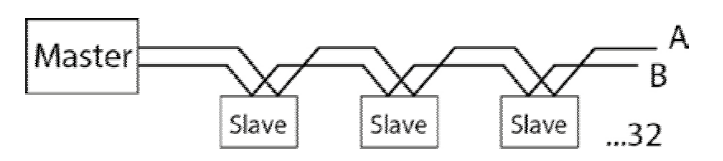
\includegraphics[scale=0.5]{pics/RS485-Schnittstelle-11.png}
\caption{Aufbau eines Modbus-Netzwerkes}
\label{fig:impl:WallboxModbusnetzwerk}
\end{figure}


\subsection{Modbus tools + libraries} \setauthor{Pouget Marcel}


Es gibt viele Tools, mit denen Daten über einen USB-zu-Modbus-Konvertieren Modbus-Register ausgelesen werden können. Für diese Arbeit wurden hauptsächlich die Programme 'QModMaster' und 'Hercules' verwendet. Es handelt sich bei beiden um kostenlose Programme. \ref{fig:impl:QmodMasterverview}


\begin{figure}[h t]
\centering
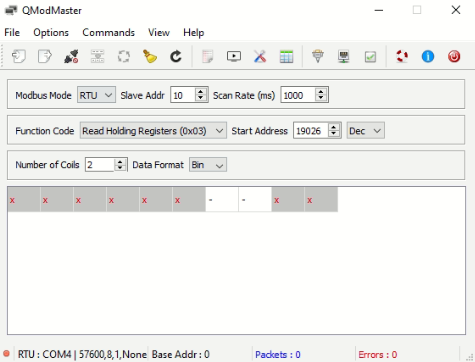
\includegraphics[scale=0.7]{pics/QmodMasterverview.png}
\caption{Overview von QModMaster }
\label{fig:impl:QmodMasterverview}
\end{figure}



In QModMaster kann bei dem Modbus-Modus zwischen dem Modus RTU und TCP gewechselt werden, da das Programm beides unterstützt. Unter der Slave Adresse kann der gewünschte Teilnehmer ausgewählt werden. Hier ist es in dem Beispiel der Slave mit der ID 10. Mit der Scan-Rate kann ein Intervall eingestellt werden, mit welchem das Tool den Port abfragt.


Bei dem Abschnitt 'Function Code' kann auswählen werden, welche Funktion \ref{tab:functionsfromModbus} ausgeführt werden soll. Die Start-Adresse ist das Register, welches beschrieben oder ausgelesen werden soll. Hier kann auch noch angegeben werden, auf welche Art die Daten übermittelt werden sollen. Es gibt die Möglichkeit für Binär-, Dezimal- und Hexadecimal-Zahlen.


Die 'Number of Coils' sagt an, wie viele Register auf einmal ausgelesen / beschrieben werden sollen, da bei manchen Geräten die Werte für ein Register zu groß sind (über 65536). In solchen Fällen werden die Daten je nach Hersteller in 2 oder mehreren Registern abgespeichert. Sollte dies der Fall sein, ist es aber immer vom Hersteller dokumentiert.



Der untere Bereich ist das Ergebnis, welches der Slave zurücksendet. Hier kann ausgewählt werden, in welcher Form die Daten angezeigt werden sollen. Ganz unten ist noch eine Zusammenfassung der Einstellungen zu sehen, wie viele Packages gesendet wurden und wie viele davon fehlerhaft waren.


\begin{figure}[h t]
\centering
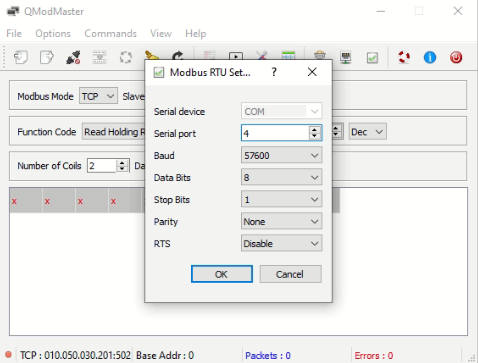
\includegraphics[scale=0.7]{pics/Settingsforqmodmaster.png}
\caption{Einstellungen für Modbus RTU}
\label{fig:impl:Settingsforqmodmaster}
\end{figure}



\ref{fig:impl:Settingsforqmodmaster} Hier können Werte der Parameter eingestellt werden. Das 'Serial-device' ist in diesem Fall der USB-Port des Computers und der 'Serial-port' ist der Steckplatz, in welchem der Modbus-Konverter steckt. Falls der Port des Adapters unbekannt ist, kann dieser in Windows unter den verbundenen Geräten im Gerätemanager gefunden werden.



'Baud' ist die Konfiguration für die Baudrate. Diese muss mit den Angaben des Herstellers übereinstimmen.



Data-Bits beschreibt die Länge des Protokolls. Dieser Wert ist auch im Datenblatt des jeweiligen Gerätes zu finden.



Die Stop-Bits sind in den Angaben des Herstellers zu finden. Der Wert beträgt meist 1 oder 2 Bits. Parity und RTS sind meist disabled, können aber bei Bedarf auch konfiguriert werden.


\begin{figure}[h t]
\centering
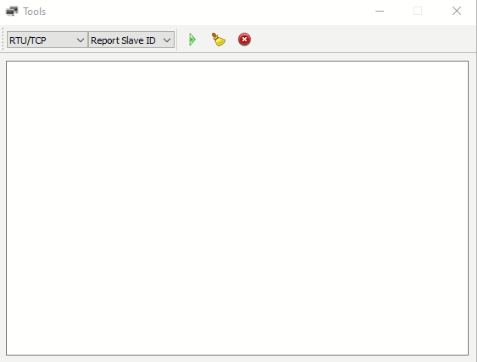
\includegraphics[scale=0.7]{pics/ToolsQModbusMaster.png}
\caption{Einstellungen für Modbus RTU}
\label{fig:impl:ToolsQModbusMaster}
\end{figure}


Außerdem gibt es einen Monitor, auf welchem die einzelnen Abfragen des Tools nachvollzogen und abspeichern werden können. Auf der \ref{fig:impl:ToolsQModbusMaster} gibt es noch weitere Tools, welche in Verbindung mit Modbus verwendet werden können.



Wenn mit QModbusMaster eine Modbus TCP Verbindung aufgebaut werden soll, muss der Modbus-Mode von RTU auf TCP eingestellt werden. Die Einstellmöglichkeiten sind fast identisch zu der Modbus RTU Verbindung, hier muss lediglich die Unit ID anstatt der SlaveID eingestellt werden, jedoch ist es derselbe Wert. \ref{fig:impl:QmodbusMasterTCP}


\begin{figure}[h t]
\centering
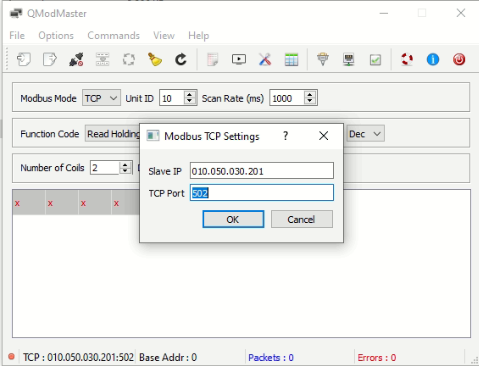
\includegraphics[scale=0.7]{pics/QmodbusMasterTCP setting.png}
\caption{Einstellungen für Modbus RTU}
\label{fig:impl:QmodbusMasterTCP}
\end{figure}


Hier ist der größte Unterschied zu der Modbus RTU. Denn anstatt der ganzen Parameter für die serielle Übertragung wird hier nur der Port und die IP-Adresse des Teilnehmers eingestellt. Der Port ist standardmäßig 502. Sollte ein anderer Port konfiguriert sein, wird dies immer in der Dokumentation des Herstellers angegeben.



\subsection{Modbus Librarys für Java }



Es gibt viele Librarys für Modbus, doch viele von ihnen bauen auf eine Schnittstelle auf, welche in C++ geschrieben wurde. Für das Projekt kam aber aufgrund der Firmenarchitektur nur ein Dependency mit einer nativen Java-Anbindung in Frage. Jlibmodbus ist ein Projekt, welches von dem Github-User kochedykov entwickelt und betreut wird. Dabei handelt es sich um ein gut dokumentiertes Projekt, welches sich einfach in jedes Maven-Projekt einbinden lässt


\begin{lstlisting}[language=java,caption=Dependency in Pom.xml,label=lst:impl:foo]
<dependency>
<groupId>com.intelligt.modbus</groupId>
<artifactId>jlibmodbus</artifactId>
<version>1.2.9.7</version>
</dependency>
\end{lstlisting}



Um die Architektur besser zu verstehen, gibt es einige Anwendungsbeispiele. Diese fassen die Bereiche von Modbus RTU, RTU over TCP oder TCP gut zusammen. Dank diesen Beispielen gab es bei der Entwicklung des Projektes keine Probleme. Auf 'sourceforge' gibt es die aktuelle Version der Library, mit welcher einfach Java-Anwendungen erweitert werden können.


\subsection{Kommunikationsaufbau zu den Wallboxen }


Bei dem Aufbau der Kommunikation zu den Wallboxen gab es die ersten Probleme der Arbeit, denn es gab für die Hardware, die genutzt wurde, keine Dokumentation. Zwar wurde von dem Hersteller der Wallboxen erklärt, welche 2 Pins für die Verkabelung von Nöten waren, jedoch gab der Hersteller des Modbus USB Konverters keine Angaben dazu, welcher der neun Pins für die Kommunikation verantwortlich ist. Dadurch wurde in den ersten Tagen der Projektarbeit sehr viel probiert, wie mithilfe des Adapters und zwei Kabeln eine Verbindung zu den Wallboxen aufgebaut werden kann. In QmodMaster wurden alle Parameter eingestellt und die Signale erfolgreich losgeschickt (dies wurde durch ein Blinken einer LED gekennzeichnet), jedoch bekam die Wallbox das Paket nie und so wurde immer ein Fehler in QModbusMaster geworfen. Erst nach dem Versuch, einfach alle neun Kabel anzuschließen und jedes Paar nacheinander zu testen, konnte festgestellt werden, dass nur durch Pin 1 und Pin 2 die Signale gesendet wurden. Doch laut Internetrecherchen hätten es Pin 5 und 6 sein müssen. Dadurch konnte die erste Verbindung mit der Wallbox, welche extra für die Modbus-Tests wieder abmontiert wurde, aufgebaut werden.




Zuerst wurden die vom Hersteller angegebenen Register-Adressen getestet und die zurückgegebenen Werte mit den Erwartungswerten verglichen. Nachdem auch das Setzen der Ladestromvorgabe erfolgreich getestet wurde, war die erste Testphase abgeschlossen. Nach dem Zusammenbau der Wallbox und der erneuten Installation wurden die Wallboxen das erste Mal an den Autos getestet. Nach erfolgreicher erster Kommunikation wurde der Modbus-zu-USB-Adapter endgültig an das Kabel für die Kommunikation angelötet. Um erste, wirklich brauchbare Daten aus den Wallboxen zu bekommen und dynamisch alle 5 Wallboxen testen zu können, wurde ein kleines, eigenes Modbus-Tool entwickelt, welches mit Java und dem JlibModbus für Linux entwickelt wurde. Dieses Tool war nur dafür gedacht, die einzelnen 5 Wallboxen ansprechen zu können und mögliche Fehler direkt zu beheben. Das Tool war ein einfaches Interface, auf welchem die ID der jeweiligen Wallbox ausgewählt werden konnte, die Registeradresse eingeben und zwischen Lesen oder Schreiben entscheiden konnte. Dadurch wurde dann auch der Effekt auf die Autos und somit auch auf die Wallboxen überprüft. Nachdem die von dem Tool vorgegebenen Werte dem entsprachen, was das Auto als Ladegeschwindigkeit anzeigte, waren die Tests erfolgreich abgeschlossen. Der nächste Schritt war es, in einem Schaltschrank, durch den auch die Stromkabel der Wallboxen liefen, einen Raspberry Pi 4 zu montieren und korrekt an das Stromnetz anzuschließen. Dieser bekam von einem Mitarbeiter der Firma die IP 10.50.30.101 zugewiesen, mit welcher er dann via SSH erreichbar war. Durch das Linux-basierte Commandoline-Tool Modpoll wurde überprüft, ob auch außerhalb der Testumgebung die Kommunikation korrekt funktioniert. Nachdem dies der Fall war, konnte es an die Entwicklung der Tasks gehen.


\subsection{Kommunikationsaufbau zu der Fronius PV Anlage }
Hier gestaltete sich die ganze Angelegenheit etwas schwerer, da es sich um eine Modbus TCP-Schnittstelle handelte. Und da hier die Dokumentation für JLibModbus nicht ganz so gut war wie für Modbus RTU, dauerte der Verbindungsaufbau etwas länger. Der Wechselrichter, welcher die Kommunikation ermöglicht, bekam bei der Installation der Anlage die IP 20.50.30.200.


Der erste Aufbau zur Anlage folgte über QModbusMaster, welcher sich als reibungslos herausstellte. Der Port 502 war in der Dokumentation des Wechselrichters zu finden. Doch bei der Suche nach der richtigen Register-Adresse fingen die Probleme an. Denn die Liste der Register war unübersichtlich, und es dauerte wirklich lange, um das Register zu finden, in welchem der aktuelle Wert der Stromproduktion gespeichert wird. Und als dann endlich die richtigen Werte zurückgeliefert wurden, trat schon das nächste Problem auf.


Denn egal, wie viel Strom die PV gerade produzierte (dies konnte immer mit der Onlineanzeige des Wechselrichters überprüft werden, welche auf der Seite der Anlage aufgerufen werden konnte. Dafür muss die IP des Wechselrichters in den Browser eingegeben werden), der Wert wurde nie größer als 65536. Nach einiger Recherche und einer Anfrage in einem Photovoltaik-Forum (\url{https://www.photovoltaikforum.com/thread/179595-auslesen-der-aktuellen-gesammtleistung-via-modbus-tcp/?pageNo=1}) wurde das Problem gefunden. Denn in der Dokumentation waren 2 Register angegeben. Das erste wurde standardmäßig gefüllt, doch wenn es seine maximale Größe von 65536 überschritt, wurde das zweite Register um einen Zähler erhöht und das erste Register auf Null gesetzt. Das bewirkt, dass eine deutlich höhere Zahl abgespeichert werden konnte und somit immer ein korrekter Wert bei einer Anfrage zurückkommt.


\subsection{Kommunikationsaufbau zu den Janitza Klemmen: } \label{text:Janitza}


Die Kommunikation zu den Janitza-Klemmen besteht aus denselben Einstellungen wie bei der Fronius-Anlage. Die IP-Adresse der Klemmen ist 10.50.30.201. Auch hier gibt es eine Website, auf welcher die Daten der Klemme überprüft werden können, somit konnte direkt überprüft werden, ob die Daten, welche ausgelesen wurden, stimmen. Auch hier gab es wieder mit den Rückgabewerten Probleme, da der Wert als FLoat angegeben wurde und es keine Angaben dazu gab, wie der Wert wieder in einen Integer zurückwandeln werden konnte. Aber zum Glück gab es in einem Beitrag in dem Forum Stack Overflow eine Anleitung dazu, wie mithilfe einer Umrechnung die richtigen Werte ausgelesen werden können.


Nach einem Abgleich zwischen den Werten des Modbus-Tools und der Webanzeige konnte eine Richtigkeit der Daten gewährleistet werden. Aus einem Abgleich der verschiedenen Daten aus dem Wechselrichter und den Messklemmen ergibt sich dann der Verbrauch der Firma. Ist der Wert der Janitza-Klemme im negativen Bereich, verbrauchen die Anlagen der Firma mehr, als die Fronius PV generieren kann. Dies ist vor allem dann der Fall, wenn es sehr bewölkt ist oder die Sonne nicht am Himmel steht. Ansonsten ist der Wert der Janitza-Klemme meist über 50 kWh, was das automatische Laden der E-Autos ermöglicht.


